% 第2章
\chapter{MPCによる歩行パターン生成}
\section{緒言}
 本章では二足歩行ロボットの歩行パターン生成に関する基本的な概念,及び提案手法について述べる.

\section{歩行(walk)}


\section{ZMP}
 二足歩行ロボットの安定性判別の指標として代表的なものとして, Vukobratović らによって提案された Zero Moment Point (以下, ZMP ) [1] がある. 以下の図\ref{Fig:Definition of Zero-Moment Point}はロボットの足部における力の分布例である.足部の境界の内側に存在する点に作用する等価な力Rとしてまとめられる.力ベクトルRが通過するこの作用点がZMPの位置である.


\begin{figure}[H]
  \centering
 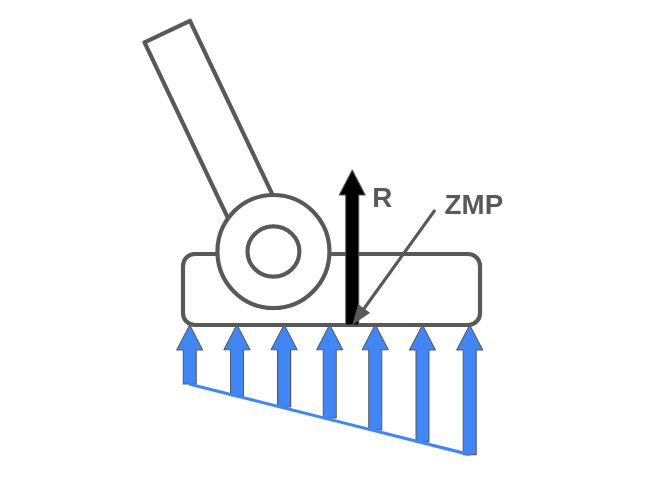
\includegraphics[keepaspectratio, scale=0.4]
      {images/walk/zmp.png}
 \caption{Definition of Zero-Moment Point}
 \label{Fig:Definition of Zero-Moment Point}
\end{figure}

 ZMPと関連する概念として支持多角形がある.
図に示すようにロボットが床面に接触している点で囲った範囲を支持多角形と考える.
この範囲に重心位置及びZMPがあれば,静的安定であり転倒しない.ZMPは常に支持多角形の中に存在する関係である.

\begin{figure}[H]
     \centering
    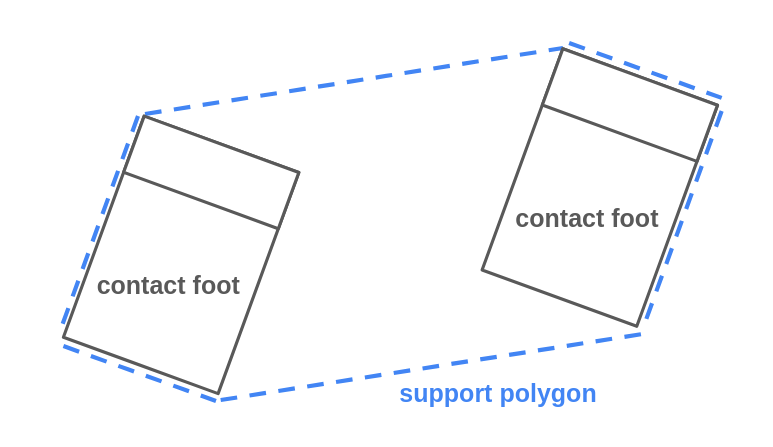
\includegraphics[keepaspectratio, scale=0.4]
         {images/walk/support_polygon.png}
    \caption{Support Polygon}
    \label{Fig:Support Polygon}
\end{figure}

%---------------------------------------
\section{テーブル台車モデル(Table-cart model)}
二足歩行ロボットのモデル化手法として,図\ref{Fig:Illustration of Table-cart model}に示すようなテーブル・台車モデルがある.質量の無視できるテーブルの上に質量Mをもつ台車が水平に走行できると考える.テーブルの台座が台車の走行範囲に比べて狭いため,台車がテーブルの端に達すると全体が転倒してしまうが,台車が適切な加速を行えば転倒を防ぐことができる.\\
このモデルから式(\ref{eq:zmp})のダイナミクスを導ける.ここでは,$x$, $\ddot{x}$はロボットの重心位置と重心加速度,$hCoM$は鉛直方向の重心の高さ,$g$は重力加速度,$p$はZMPの位置である.式(\ref{eq:zmp})によるモデル化に対し,システムへの入力を台車の重心の躍度(jerk),$\dddot{x}$とおくと,式(\ref{eq:system1}),式(\ref{eq:system2})のようなシステムとして表現できる.

%テーブル台車では重心の運動によってZMPが発生する因果関係を前提とすると,目標とするZMP軌道を定めてからこれを実現する安定な重心運動を計算する手順の歩行パターンの手法をZMPを規範とする歩行パターン生成法という.

\begin{equation}
     p=x-\frac{h_{CoM}}{g}\ \ddot{x}
     \label{eq:zmp}
\end{equation}

\begin{equation}
     \frac{d}{dt}\left(\begin{matrix}x\\\dot{x}\\\ddot{x}\\\end{matrix}\right)=\left(\begin{matrix}0&1&0\\0&0&1\\0&0&0\\\end{matrix}\right)\left(\begin{matrix}x\\\dot{x}\\\ddot{x}\\\end{matrix}\right)+\left(\begin{matrix}0\\0\\1\\\end{matrix}\right)u
     \label{eq:system1}
\end{equation}

\begin{equation}
     p=\left(\begin{matrix}1&0&-\frac{h_{CoM}}{g}\ \\\end{matrix}\right)\left(\begin{matrix}x\\\dot{x}\\\ddot{x}\\\end{matrix}\right)
     \label{eq:system2}
\end{equation}

ここで,上記のシステムを離散化すると,システムは式(\ref{eq:2.4})\~{}(\ref{eq:2.6})で表すことができる.

\begin{equation}
     \widehat{x}_k=\left(\begin{matrix}x\left(kT\right)\\\dot{x}\left(kT\right)\\\ddot{x}\left(kT\right)\\\end{matrix}\right),u_k=\dddot{x}\left(kT\right),z_k=z\left(kT\right)
     \label{eq:2.4}
\end{equation}

\begin{equation}
     \widehat{x}_{k+1}=\left(\begin{matrix}1&T&T^2/2\\0&1&T\\0&0&1\\\end{matrix}\right)\widehat{x}_k+\left(\begin{matrix}T^3/6\\T^3/2\\T\\\end{matrix}\right)u_k
     \label{eq:2.5}
\end{equation}

\begin{equation}
     z_k=\left(\begin{matrix}1&0&-\frac{h_{CoM}}{g}\ \\\end{matrix}\right)\widehat{x}_k
     \label{eq:2.6}
\end{equation}

\begin{figure}[H]
  \centering
 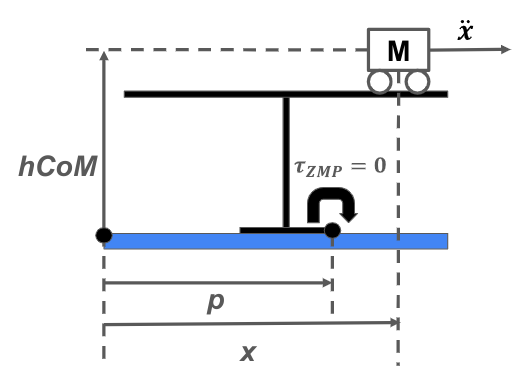
\includegraphics[keepaspectratio, scale=0.5]
      {images/walk/table.png}
 \caption{Illustration of Table-cart model}
 \label{Fig:Illustration of Table-cart model}
\end{figure}

% -----------------------------------------------------------
\section{予見制御による歩行パターン生成手法}
上記の ZMP とテーブル台車モデルの概念を利用した歩行パターン生成手法としては,kajita らによる予見制御を利用した歩行パターン生成手法 [2] がある. kajita らによる手法では (2.4)˜(2.6) で表現したロボットのダイナミクスに対して,予見制御理論によって以下の評価関数式 (2.7) を最小化する制御入力(二足歩行ロボットの歩行パターン)を得る.


\begin{equation}
     \min_{\substack{{\dddot{x}}_k,\ {\dddot{x}}_{k+1},\ \cdots}} \sum_{i=k}^{\infty}\left(\frac{1}{2}Q\left(z_{i+1}-z_{i+1}^{ref}\right)^2\ +\ \frac{1}{2}R{\dddot{x}}_i^2\right)
\end{equation}


式 (2.7) 内, z は ZMP の位置, z ref は ZMP の目標位置, u は入力である重心の躍度( jerk ),Q と R は重みを示す.
%---------------------------------------------------------------
\section{MPCを利用した歩行パターン生成手法}
本研究では, kajita らによる予見制御を利用した歩行パターン生成手法 [2] を MPC によって拡張した, Wieber らによる手法 [3] を実装する.ここでは,その手法 [3] について紹介する.
まず, MPC は最適制御の一種であり,無限長の区間に渡る最適化問題を解く代わりに,有限長の区間で最適化問題を解いて最適入力を得る手法である.有限区間の最適化問題であるがゆえに,陽に表現した制約を考慮しながら最適化問題を解くことができるのが特徴である.また,有限区間での最適化問題を解く際には,有限区間に渡る未来の状態,ないしは出力の予測値を利用して最適化を行う.式 (2.8) で表されるダイナミクスからなる一般的なシステムでは,状態の予測は式 (2.9) で表される

\begin{equation}
     \left\{\begin{aligned}\dot{x} &= Ax + Bu \\ y &= Cx \\\end{aligned}\right.
\end{equation}

\begin{equation}
     \left(\begin{matrix}x_{k+1}\\x_{k+2}\\x_{k+3}\\\vdots\\x_{k+n}\\\end{matrix}\right)=\left(\begin{matrix}A\\A^2\\A^3\\\vdots\\A^n\\\end{matrix}\right)x_k+\left(\begin{matrix}B&0&\cdots&&0\\AB&B&0&\cdots&0\\A^2&AB&B&\cdots&0\\\vdots&\vdots&&&0\\A^{n-1}B&A^{n-2}B&\cdots&AB&B\\\end{matrix}\right)\left(\begin{matrix}u_k\\u_{k+1}\\u_{k+2}\\\vdots\\u_{k+n-1}\\\end{matrix}\right)
\end{equation}

\begin{equation}
     C=\left(\begin{matrix}C&0&\cdots&0\\0&C&\cdots&0\\\vdots&&\ddots&0\\0&\cdots&&C\\\end{matrix}\right)
\end{equation}

\begin{equation}
     \left(\begin{matrix}z_{k+1}\\z_{k+2}\\z_{k+3}\\\vdots\\z_{k+n}\\\end{matrix}\right)=\left(\begin{matrix}C&0&\cdots&0\\0&C&\cdots&0\\\vdots&&\ddots&0\\0&\cdots&&C\\\end{matrix}\right)\left(\begin{matrix}x_k\\x_{k+1}\\x_{k+2}\\\vdots\\x_{k+n-1}\\\end{matrix}\right)
\end{equation}

\begin{equation}
     \min_{\substack{{\dddot{x}}_k,\ {\dddot{x}}_{k+1},\ \cdots,\ {\dddot{x}}_{k+n}}} \sum_{i=k}^{n}\left(\frac{1}{2}Q\left(z_{i+1}-z_{i+1}^{ref}\right)^2\ +\ \frac{1}{2}R{\dddot{x}}_i^2\right)
\end{equation}

\begin{equation}
     \left(\begin{matrix}L_{u_0}\\\vdots\\L_{u_n}\\\end{matrix}\right)\le\dddot{x}\le\left(\begin{matrix}U_{u_0}\\\vdots\\U_{u_n}\\\end{matrix}\right)
\end{equation}

\begin{equation}
     \left(\begin{matrix}L_{x_0}\\\vdots\\L_{x_n}\\\end{matrix}\right)\le z\le\left(\begin{matrix}U_{x_0}\\\vdots\\U_{x_n}\\\end{matrix}\right)
\end{equation}

\newpage